\section{Estado del Arte}

\subsection{2.1. Técnicas Tradicionales de Asignación de Recursos}

Aunque los métodos clásicos de optimización han servido de base durante años en sistemas satelitales, su rigidez se vuelve evidente al confrontarlos con la dinámica implacable de las NTN. Enfoques basados en programación lineal, convexa o heurísticas greedy tienden a optimizar bajo supuestos de conocimiento perfecto del canal o variabilidad lenta, condiciones que rara vez se cumplen en constelaciones LEO. 

Resulta revelador observar cómo estas técnicas logran soluciones factibles en escenarios estáticos pero degradan rápidamente ante Doppler severo, handovers frecuentes y fluctuaciones de carga. En muchos casos estudiados, priorizan un único KPI —usualmente throughput— a costa de fairness o niveles de interferencia, limitando su utilidad en redes integradas TN-NTN. 

Aygul et al. \cite{Aygul2024} destacan precisamente estas brechas al analizar la integración terrestre-no terrestre, señalando cómo los delays de propagación y la falta de adaptabilidad en tiempo real representan obstáculos persistentes que los algoritmos tradicionales apenas mitigan.

\subsection{2.2. Aplicaciones de Aprendizaje Supervisado y No Supervisado}

Particularmente llamativo es el salto que han dado las técnicas de machine learning supervisado y no supervisado para predecir patrones en entornos NTN. Modelos de regresión, redes neuronales convolucionales y clustering han demostrado utilidad en tareas de predicción de canal, clasificación de usuarios y detección de anomalías. 

No obstante, cabe matizar que estos enfoques suelen operar de manera offline o con entrenamiento periódico, lo cual reduce su efectividad ante cambios abruptos en la topología orbital. Lejos de ser un asunto resuelto, la literatura sugiere que su principal contribución radica en servir como pre-procesadores o estimadores que alimentan módulos de decisión posteriores, más que en proporcionar control autónomo completo. 

\cite{Aygul2024} revisa cómo estas herramientas facilitan la integración TN-NTN, aunque subraya limitaciones en manejo de dinámica extrema y optimización multi-objective.

\begin{figure}[h]
\centering
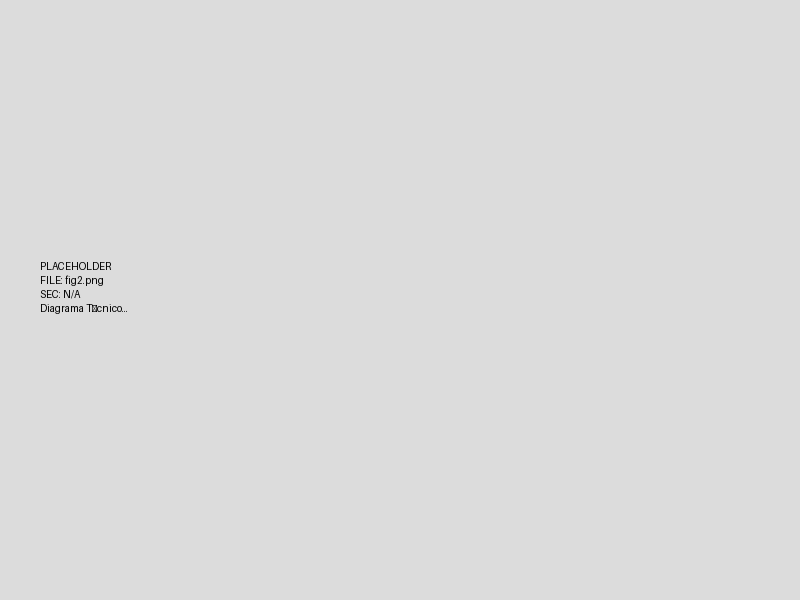
\includegraphics[width=\linewidth]{fig2.png}
\caption{Evolución temporal del número de publicaciones indexadas relacionadas con optimización de recursos en NTN mediante técnicas de inteligencia artificial (datos hasta 2025).}
\label{fig:evolucion_publicaciones}
\end{figure}

\subsection{2.3. Enfoques Basados en Reinforcement Learning}

Uno de los avances más prometedores —y al mismo tiempo más reveladores de limitaciones actuales— surge con el reinforcement learning. Agentes DRL han conseguido mejoras notables en asignación de recursos al aprender políticas directamente de la interacción con el entorno. 

Cao et al. \cite{Cao2023} proponen un esquema colaborativo de DRL de dos escalas temporales donde satélite y usuario terrestre comparten responsabilidades de decisión, logrando un balance interesante entre rendimiento y complejidad computacional. Sin embargo, su diseño black-box reduce la interpretabilidad, aspecto crítico para despliegues operativos. 

De forma similar, Mohsin et al. \cite{Mohsin2025} exploran DRL en redes TN-NTN asistidas por RIS activos, reportando ganancias significativas en throughput y mitigación de interferencias. Mientras tanto, Minani et al. \cite{Minani2025_Channel} combinan LSTM para predicción de canal con DRL para asignación fair en uplinks NTN, enfatizando la importancia de anticipación proactiva. 

Tabla 2: Resumen comparativo de trabajos representativos en optimización de recursos NTN (incluyendo enfoque, métricas principales y limitaciones identificadas).

A pesar de estos progresos, persisten brechas notables. La mayoría de soluciones DRL carecen de mecanismos robustos de guía de alto nivel, sufren de ineficiencia en entrenamiento en espacios de acción grandes y muestran vulnerabilidad ante distribuciones de usuarios no vistas durante el entrenamiento. Nuestra propuesta busca precisamente abordar estas limitaciones mediante integración de Large AI Models como guías semánticas y de razonamiento para agentes DRL multi-agente, orientados a optimización conjunta de throughput, interferencias y fairness en escenarios down-link más complejos.